\chapter{酶与表型}\label{ch:g11:enzymes-and-phenotype}

暹罗猫身体大部分呈奶油色，耳朵、口鼻、爪子和尾巴则为深棕色——
即身体较冷的部位。剃掉它背上的一小块毛，
用冰袋使这一小块皮肤保持低温，待毛发重新长出，
新长出的毛发便是深色的。这只猫的\omterm{def:g10:universal-dna:gene}{基因}并未改变；
它的色素合成酶只在 \qty{35}{\celsius} 以下起作用，高于此温度则不起作用。
在\omterm{def:g10:universal-dna:gene}{基因}与可见性状之间，几乎总有一种酶；
在酶与性状之间，则是酶发挥作用的环境。
本章讨论的正是这两个中间环节。

\section{三个层次上的表型}

\begin{definition}[基因型与表型]\label{def:g11:enzymes-and-phenotype:phenotype}
个体的\emph{基因型}\index{基因型}是其所携带的\omterm{def:g10:universal-dna:gene}{等位基因}的集合；
其\emph{表型}\index{表型}则是其可观察特征的集合。
表型可在下列
三个层次上加以描述：
\begin{itemize}
  \item \emph{分子水平}：存在哪些\omterm{def:g11:gene-expression:protein}{蛋白质}，
        以何种形式存在，具有何种活性；
  \item \emph{\omterm{def:g10:cells-common-unit:cell}{细胞}水平}：\omterm{def:g10:cells-common-unit:cell}{细胞}的形态、
        内含物及行为；
  \item \emph{个体水平}：可见性状，
        从眼睛颜色到疾病症状。
\end{itemize}
每一层次都是其下方层次的结果。
\end{definition}

\begin{example}[镰状细胞病的三个层次]\label{ex:g11:enzymes-and-phenotype:sickle}
分子水平：血红蛋白链中的一个\omterm{def:g10:chemistry-of-life:families}{氨基酸}（第 6 位的谷氨酸）被缬氨酸取代，
氧含量低时，改变后的分子相互黏连成长纤维。\omterm{def:g10:cells-common-unit:cell}{细胞}水平：
纤维使红\omterm{def:g10:cells-common-unit:cell}{细胞}变形为刚硬的镰刀状，
该形态会堵塞小血管，且易于破裂。个体水平：
贫血，血管堵塞时出现疼痛发作，脾脏与肾脏受损。
同一\omterm{def:g10:universal-dna:gene}{基因}的同一\omterm{def:g11:gene-expression:code}{密码子}上发生一次替换，
却可从三个层次描述其后果。
\end{example}

\begin{omfigure}
\begin{tikzpicture}[font=\small, >=Stealth,
  b/.style={draw, rounded corners, align=center, text width=3.4cm, minimum height=1.2cm}]
  \node[b, fill=omDef!12] (g) at (0,0) {\textbf{基因型}\\ 色素合成酶基因的 \\ 两个等位基因};
  \node[b, fill=omProp!15] (m) at (4.2,0) {\textbf{分子水平}\\ 酶有活性 \\ 或无活性};
  \node[b, fill=omProp!15] (c) at (8.4,0) {\textbf{细胞水平}\\ 色素细胞充满 \\ 黑色素或为空};
  \node[b, fill=omProp!15] (o) at (12.6,0) {\textbf{个体水平}\\ 皮肤、毛发和眼睛 \\ 是否着色};
  \draw[->] (g) -- (m); \draw[->] (m) -- (c); \draw[->] (c) -- (o);
  \node[b, fill=omMeth!15, text width=5cm] (e) at (6.3,-2.2) {\textbf{环境}\\ 温度、光照、饮食\dots};
  \draw[->] (e.north) -- (m.south);
  \draw[->] (e.north east) -- (c.south);
  \draw[->] (e.east) -| (o.south);
\end{tikzpicture}

{\small 色素形成：从\omterm{def:g11:enzymes-and-phenotype:phenotype}{基因型}到\omterm{def:g11:enzymes-and-phenotype:phenotype}{表型}。\omterm{def:g11:enzymes-and-phenotype:phenotype}{表型}的每一层次
都由其前一层次决定；环境在每一步都发挥作用，
影响酶发挥作用的程度、\omterm{def:g10:cells-common-unit:cell}{细胞}的反应方式，
以及生物体的外观。}
\end{omfigure}

\begin{proposition}[蛋白质决定表型]\label{prop:g11:enzymes-and-phenotype:proteins}
\omterm{def:g11:enzymes-and-phenotype:phenotype}{表型}的每一层次都由\omterm{def:g11:gene-expression:protein}{蛋白质}产生：\omterm{def:g10:universal-dna:gene}{等位基因}决定一种\omterm{def:g11:gene-expression:protein}{蛋白质}
（见\cref{ch:g11:gene-expression}）；\omterm{def:g11:gene-expression:protein}{蛋白质}的活性决定\omterm{def:g10:cells-common-unit:cell}{细胞}的
化学过程与结构；\omterm{def:g10:cells-common-unit:cell}{细胞}决定
生物体的性状。其中大多数\omterm{def:g11:gene-expression:protein}{蛋白质}是\emph{酶}，
因此多数性状是一连串酶促反应
的结果。
\end{proposition}
\admitted

\section{酶}

\begin{definition}[酶、底物、活性位点]\label{def:g11:enzymes-and-phenotype:enzyme}
称\emph{酶}\index{酶}为一种催化单一化学反应的\omterm{def:g11:gene-expression:protein}{蛋白质}：它能使
该反应的速率提高数百万倍，而自身并不被消耗。
被酶转化的分子称为其\emph{底物}\index{底物}；
反应发生在酶的一个凹穴中，
即\emph{活性位点}\index{活性位点}，其形状与化学性质
只与该底物相匹配，而与其他分子不符。
这种\emph{专一性}源于酶的三维折叠结构，
进而取决于其\omterm{def:g10:chemistry-of-life:families}{氨基酸}序列，最终由其\omterm{def:g10:universal-dna:gene}{基因}决定。
\end{definition}

\begin{omfigure}
\begin{tikzpicture}[font=\small, >=Stealth]
  % enzyme with a notch (active site)
  \draw[thick, fill=omDef!15, rounded corners=10pt] (0,0) -- (3.2,0) -- (3.2,2.4) -- (2.2,2.4) -- (2.2,1.5) -- (1.4,1.5) -- (1.4,2.4) -- (0,2.4) -- cycle;
  \node at (1.6,0.7) {酶};
  \node[font=\scriptsize, anchor=east] at (1.25,2.75) {活性位点};
  \draw[gray] (1.3,2.75) -- (1.6,2.3);
  % fitting substrate
  \draw[thick, fill=omMeth!40] (4.6,3.3) rectangle (5.4,4.1);
  \node[font=\scriptsize, anchor=west] at (5.55,3.7) {底物A：可契合};
  \draw[->, thick] (4.5,3.4) -- (2.1,2.6);
  % non-fitting substrate
  \draw[thick, fill=omThm!35] (4.6,1.6) -- (5.6,1.6) -- (5.1,2.5) -- cycle;
  \node[font=\scriptsize, anchor=west] at (5.7,2.0) {底物B：不契合};
  \draw[->, thick, omThm] (4.5,1.9) -- (3.5,2.2);
  \draw[thick, omThm] (3.25,2.0) -- (3.55,2.4); \draw[thick, omThm] (3.25,2.4) -- (3.55,2.0);
  % products
  \node[anchor=west, align=left] at (7.5,0.4) {A 转化为其产物；\\ B 保持不变。};
\end{tikzpicture}

{\small 专一性。\omterm{def:g11:enzymes-and-phenotype:enzyme}{活性位点}是为某一\omterm{def:g11:enzymes-and-phenotype:enzyme}{底物}而成形的凹穴；
另一种形状的分子无法结合，因而不会被转化。
改变凹穴的形状——如由\omterm{def:g11:mutations:mutation}{突变}所致——则
酶会失去或改变其\omterm{def:g11:enzymes-and-phenotype:enzyme}{底物}。}
\end{omfigure}

\begin{example}[乳糖酶]\label{ex:g11:enzymes-and-phenotype:lactase}
乳糖，即乳汁中的糖，在小肠内壁乳糖酶的作用下
被分解为两个单糖；若不被分解，
则会未经消化进入结肠，细菌在那里将其\omterm{def:g10:cell-metabolism:fermentation}{发酵}，
引起胀气、腹部痉挛和腹泻。所有婴儿都能合成乳糖酶；但在大多数人类中，
其\omterm{def:g10:universal-dna:gene}{基因}在断奶后即被关闭，成人即为乳糖不耐受者。
在有着悠久乳制品生产历史的人群中，
一种可使该\omterm{def:g10:universal-dna:gene}{基因}终生保持活性的\omterm{def:g10:universal-dna:gene}{等位基因}十分常见——在北欧为 90\%，
在东亚为 10\%。出售给乳糖不耐受者的乳糖酶滴剂，
含有相同的酶，由真菌制成。
\end{example}

\begin{omfigure}
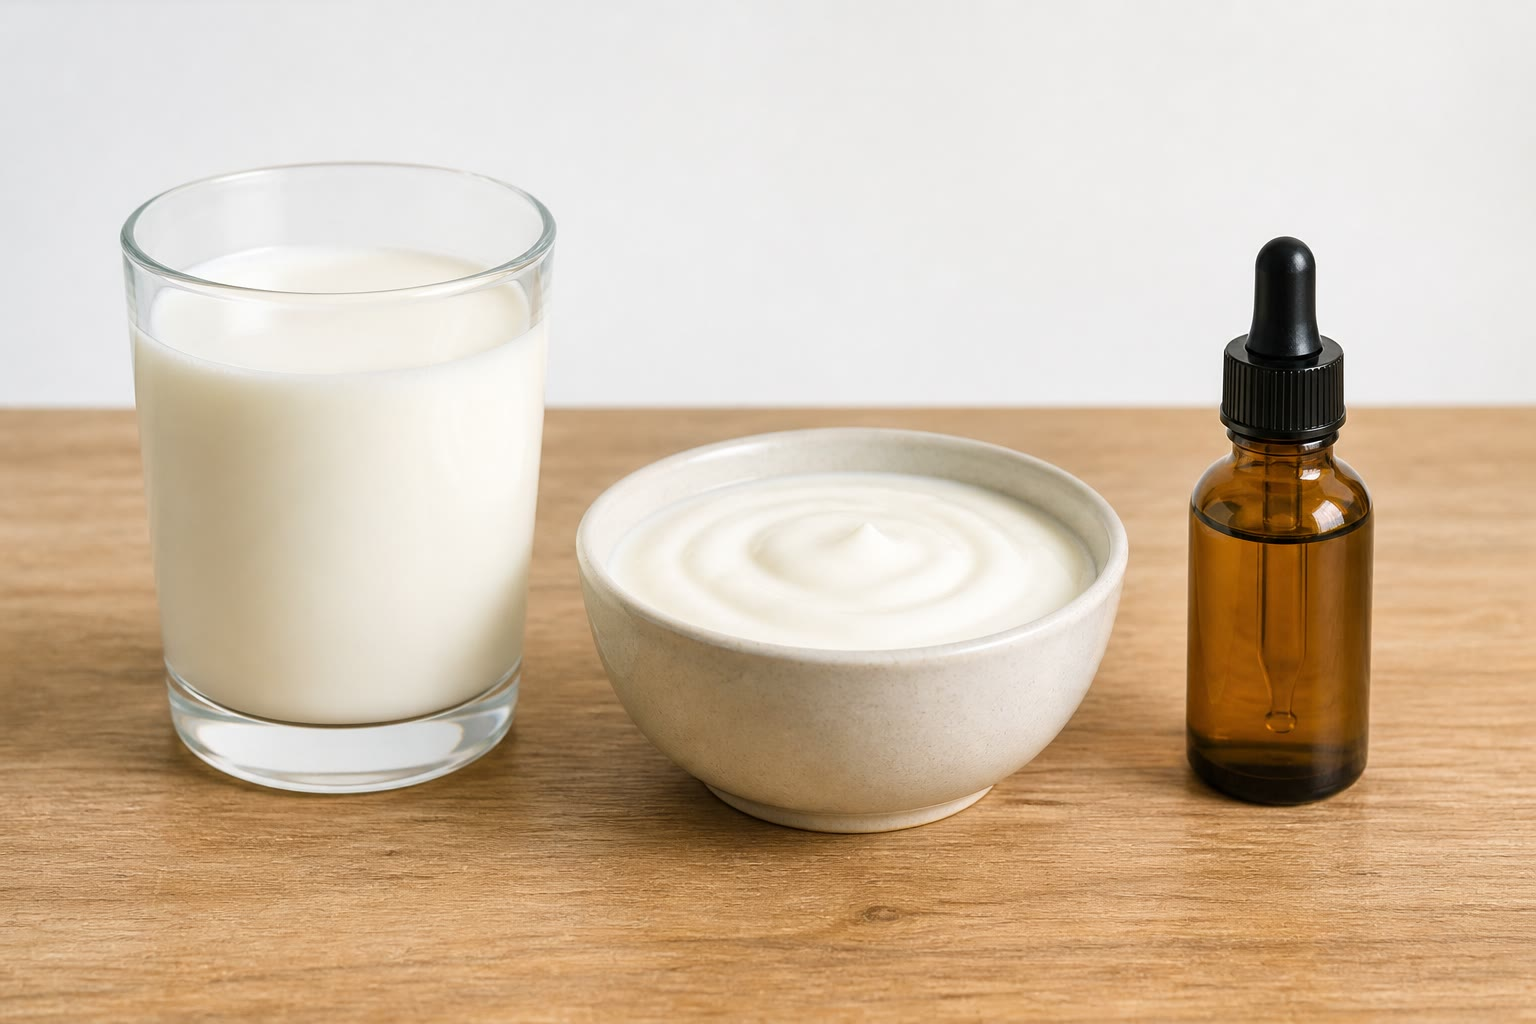
\includegraphics[width=0.58\linewidth]{images/book2/ai/g11-enzyme-lactase-milk.jpg}

{\small 牛奶、酸奶和一瓶乳糖酶滴剂。成人能否消化牛奶
取决于一个\omterm{def:g10:universal-dna:gene}{等位基因}；酸奶中的细菌已分解大部分乳糖；滴剂
补充了肠道所缺的
酶。}
\end{omfigure}

\begin{proposition}[活性条件]\label{prop:g11:enzymes-and-phenotype:conditions}
酶的活性取决于外界环境。它随温度升高而上升，
直至\omterm{def:g11:gene-expression:protein}{蛋白质}开始变性，随后急剧下降——
人体酶在 \qty{37}{\celsius} 附近活性最高，温度超过约
\num{45} 时即被破坏；每种酶只在与其所在位置相适应的酸碱度范围内起作用
（胃蛋白酶适于胃中的酸性环境，胰蛋白酶适于中性的肠道）；
其反应速率随\omterm{def:g11:enzymes-and-phenotype:enzyme}{底物}浓度升高而增大，直至达到最大值，
此时每个\omterm{def:g11:enzymes-and-phenotype:enzyme}{活性位点}都被占用。
\end{proposition}
\admitted

\begin{omfigure}
\begin{tikzpicture}
\begin{axis}[
  width=0.45\linewidth, height=5cm,
  axis x line=bottom, axis y line=left,
  xmin=0, xmax=60, ymin=0, ymax=110,
  xlabel={温度 (\unit{\celsius})}, ylabel={活性 (\%)},
  xlabel style={font=\small, at={(axis description cs:0.5,-0.15)}, anchor=north},
  ylabel style={font=\small},
  tick label style={font=\small}, xtick={0,10,20,30,40,50,60}, ytick={0,50,100},
  clip=false,
]
\addplot[thick, omThm, smooth] coordinates {(0,3) (10,10) (20,30) (30,65) (37,100) (41,85) (45,35) (50,5) (55,0)};
\end{axis}
\begin{axis}[
  xshift=0.5\linewidth,
  width=0.45\linewidth, height=5cm,
  axis x line=bottom, axis y line=left,
  xmin=0, xmax=12, ymin=0, ymax=110,
  xlabel={pH}, ylabel={活性 (\%)},
  xlabel style={font=\small, at={(axis description cs:0.5,-0.15)}, anchor=north},
  ylabel style={font=\small},
  tick label style={font=\small}, xtick={0,2,4,6,8,10,12}, ytick={0,50,100},
  legend style={at={(0.5,-0.42)}, anchor=north, legend columns=2, font=\small, draw=none},
  clip=false,
]
\addplot[thick, omDef, smooth] coordinates {(0,20) (1,70) (2,100) (3,70) (4,20) (5,3) (6,0)};
\addplot[thick, omMeth, smooth] coordinates {(5,0) (6,20) (7,70) (8,100) (9,70) (10,20) (11,3)};
\legend{胃蛋白酶（胃）, 胰蛋白酶（肠道）}
\end{axis}
\end{tikzpicture}

{\small 左图：人体酶的活性随温度变化的曲线——先上升，
在 \qty{37}{\celsius} 附近达到峰值，随后因受热而被破坏。右图：
两种消化酶，各自只在其所在器官的
酸碱度下有活性。}
\end{omfigure}

\section{反应链}

\begin{proposition}[代谢途径]\label{prop:g11:enzymes-and-phenotype:pathway}
\omterm{def:g10:cells-common-unit:cell}{细胞}很少只经一步就生成产物：起始分子
经一系列酶的作用逐步转化，每种酶作用于前一步的产物，
沿一条\emph{代谢途径}\index{代谢途径}进行。
每种酶由各自的\omterm{def:g10:universal-dna:gene}{基因}编码。任一酶的无功能\omterm{def:g10:universal-dna:gene}{等位基因}
都会在相应步骤阻断该途径：产物不能生成，
而被阻断的酶所作用的\omterm{def:g11:enzymes-and-phenotype:enzyme}{底物}可能积累。两个不同的\omterm{def:g10:universal-dna:gene}{基因}
因此可以产生相同的可见缺陷，而一个\omterm{def:g10:universal-dna:gene}{基因}的缺陷
也可能引起多种缺陷。
\end{proposition}
\admitted

\begin{omfigure}
\begin{tikzpicture}[font=\small, >=Stealth,
  mol/.style={draw, rounded corners, fill=omDef!10, minimum height=0.8cm, text width=2.2cm, align=center}]
  \node[mol] (phe) at (0,0) {苯丙氨酸 \\ （来自食物）};
  \node[mol] (tyr) at (3.6,0) {酪氨酸};
  \node[mol] (dopa) at (7.2,0) {DOPA};
  \node[mol, fill=gray!30] (mel) at (10.8,0) {黑色素 \\ （色素）};
  \draw[->, thick] (phe) -- node[above=5pt, font=\scriptsize, align=center] {酶 1\\ （肝脏）} (tyr);
  \draw[->, thick] (tyr) -- node[above=5pt, font=\scriptsize, align=center] {酶 2\\ （酪氨酸酶）} (dopa);
  \draw[->, thick] (dopa) -- node[above=5pt, font=\scriptsize, align=center] {其他 \\ 酶} (mel);
  \node[draw, fill=omThm!12, rounded corners, align=center, text width=3.2cm] (pku) at (1.8,-1.9) {缺少酶 1:\\ 苯丙酮尿症};
  \draw[->, omThm, thick] (pku.north) -- (1.8,-0.35);
  \draw[thick, omThm] (1.55,-0.2) -- (2.05,0.2); \draw[thick, omThm] (1.55,0.2) -- (2.05,-0.2);
  \node[draw, fill=omThm!12, rounded corners, align=center, text width=3.2cm] (alb) at (5.4,-1.9) {缺少酶 2:\\ 白化病};
  \draw[->, omThm, thick] (alb.north) -- (5.4,-0.35);
  \draw[thick, omThm] (5.15,-0.2) -- (5.65,0.2); \draw[thick, omThm] (5.15,0.2) -- (5.65,-0.2);
  \node[anchor=west, font=\scriptsize, align=left] at (7.2,-1.9) {苯丙氨酸在血液中积累，\\ 造成脑损伤，\\ 除非饮食中不含该物质};
\end{tikzpicture}

{\small 同一途径，两种疾病。酶 1 受阻，使
苯丙氨酸积累（苯丙酮尿症）；酶 2 受阻，
使色素无法生成（白化病）。两者均为隐性：一个有功能的\omterm{def:g10:universal-dna:gene}{等位基因}
即可提供足够的酶。}
\end{omfigure}

\begin{example}[苯丙酮尿症，以及饮食如何改变表型]\label{ex:g11:enzymes-and-phenotype:pku}
约每一万名新生儿中有一人携带两个无功能的
酶 1 \omterm{def:g10:universal-dna:gene}{基因}\omterm{def:g10:universal-dna:gene}{等位基因}。食物中的苯丙氨酸不能被转化；
其在血液中的浓度升高至二十倍，并毒害
发育中的大脑。若不治疗，患儿将出现严重的智力
障碍。出生时，经由滴在卡片上的一滴血检出——所有
新生儿均接受检测——并改用几乎不含苯丙氨酸的饮食，
该患儿即可正常发育。\omterm{def:g11:enzymes-and-phenotype:phenotype}{基因型}并未改变；\omterm{def:g11:enzymes-and-phenotype:phenotype}{表型}
在分子水平以上的各个层次，都与健康人无异。
起决定作用的是环境，此处指饮食。
\end{example}

\begin{omfigure}
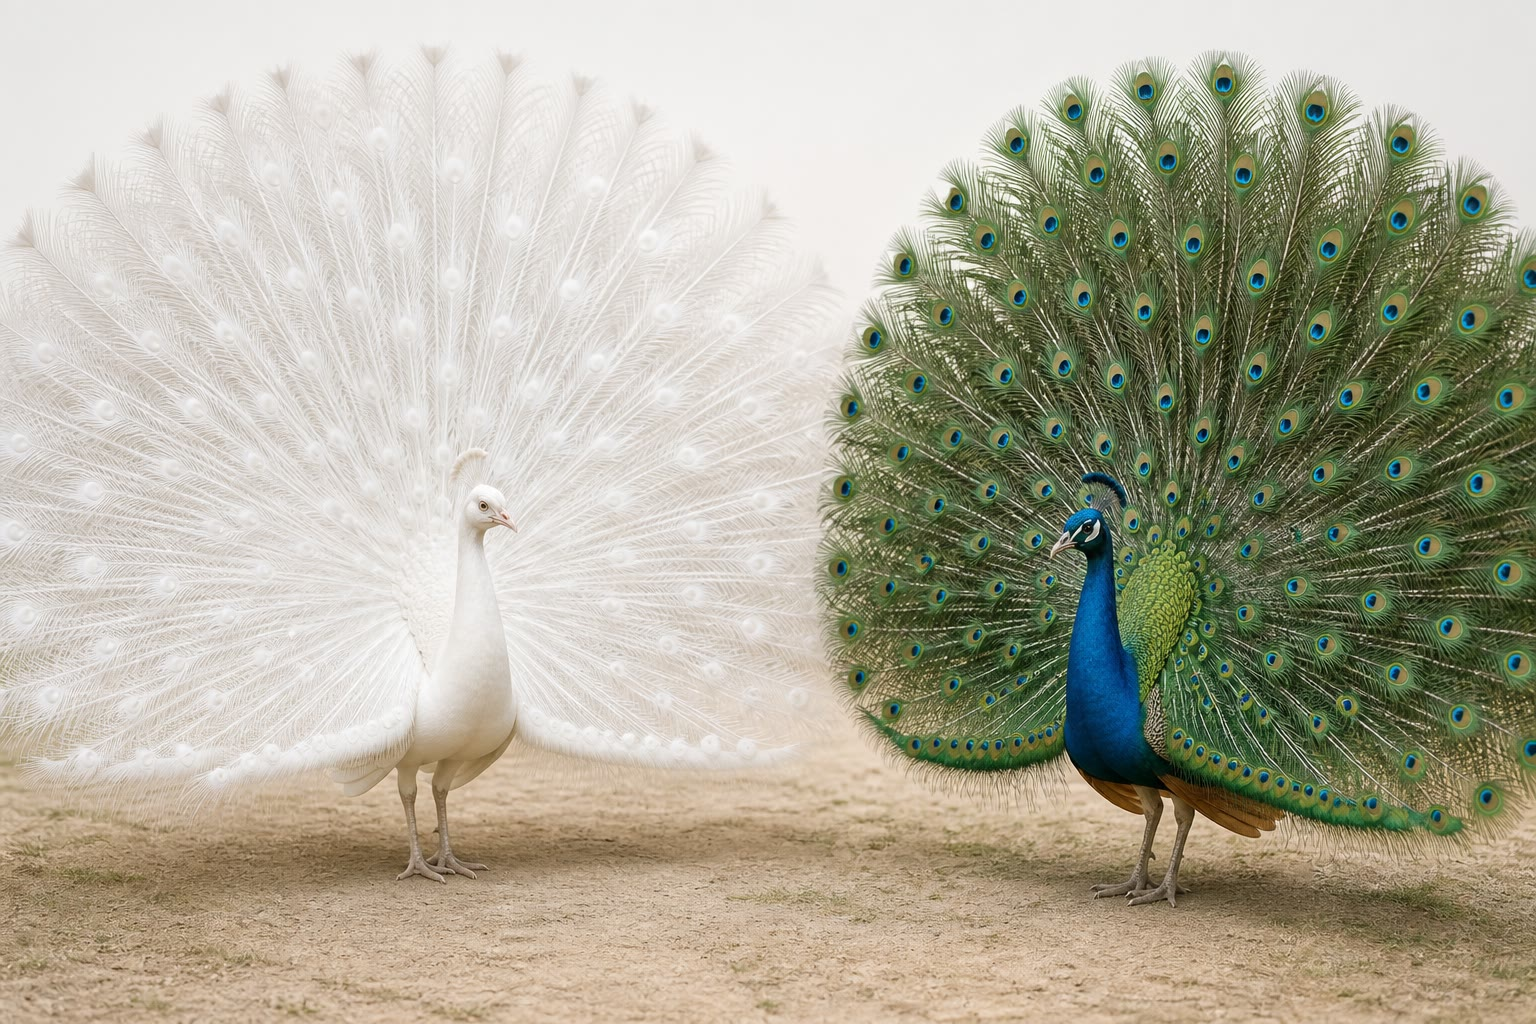
\includegraphics[width=0.6\linewidth]{images/book2/ai/g11-phenotype-albino-peacock.jpg}

{\small 一只白化孔雀与一只普通孔雀并排。酪氨酸酶\omterm{def:g10:universal-dna:gene}{基因}的两个
无功能\omterm{def:g10:universal-dna:gene}{等位基因}：酶缺失，色素\omterm{def:g10:cells-common-unit:cell}{细胞}
中空无物，每根羽毛都是白色的，
与人类白化病在三个层次上的情形一致。}
\end{omfigure}

\section{基因型、环境与表型}

\begin{proposition}[环境塑造表型]\label{prop:g11:enzymes-and-phenotype:environment}
\omterm{def:g11:enzymes-and-phenotype:phenotype}{表型}是\omterm{def:g11:enzymes-and-phenotype:phenotype}{基因型}\emph{与}环境共同作用的结果。环境
作用于分子水平（温度和酸碱度影响酶的活性，
\omterm{def:g11:enzymes-and-phenotype:enzyme}{底物}是否存在决定某条途径能否进行），
作用于\omterm{def:g10:cells-common-unit:cell}{细胞}水平（\omterm{def:g10:cells-common-unit:cell}{细胞}对
信号、营养物质和光作出反应），也作用于个体水平
（饮食、运动、疾病）。\omterm{def:g11:enzymes-and-phenotype:phenotype}{基因型}相同的个体——
同卵双胞胎、同一植株的扦插枝条——
会因各自的经历而\omterm{def:g11:enzymes-and-phenotype:phenotype}{表型}不同；\omterm{def:g11:enzymes-and-phenotype:phenotype}{基因型}不同的个体，
在适宜的条件下，也可能表现出相同的\omterm{def:g11:enzymes-and-phenotype:phenotype}{表型}。
\end{proposition}
\begin{proof}[证据]
暹罗猫的酪氨酸酶对温度敏感：色素
仅在较冷的末端形成，经冷却的剃毛部位会重新长出深色毛。
苯丙酮尿症可通过饮食加以控制。同卵双胞胎分开抚养，
身高相差数厘米，体重相差更多。
同一无性系植株分别种植在海平面和高海拔地区，
株高相差十倍，移植后又恢复原状。在每一个
例子中，\omterm{def:g11:enzymes-and-phenotype:phenotype}{基因型}固定不变，\omterm{def:g11:enzymes-and-phenotype:phenotype}{表型}随
条件而变化。
\end{proof}

\begin{method}[由基因推断性状]\label{met:g11:enzymes-and-phenotype:reason}
\begin{enumerate}
  \item 确定\omterm{def:g11:gene-expression:protein}{蛋白质}：是哪种酶、属于哪条途径，
        以及它的作用。
  \item 确定\omterm{def:g10:universal-dna:gene}{等位基因}对\omterm{def:g11:gene-expression:protein}{蛋白质}的影响：正常、减弱、
        缺失，或活性条件发生改变。
  \item 沿层次向上追踪后果：\omterm{def:g10:cells-common-unit:cell}{细胞}缺少或积累了什么，
        再看个体表现出什么。
  \item 询问需要多少个有功能的\omterm{def:g10:universal-dna:gene}{等位基因}：对大多数酶而言，一个即已足够，
        因此只有两个无功能的\omterm{def:g10:universal-dna:gene}{等位基因}时，缺陷才会出现
        （即隐性性状）。
  \item 询问环境又带来什么影响：\omterm{def:g11:enzymes-and-phenotype:enzyme}{底物}是否存在，
        温度如何，是否进行治疗。
\end{enumerate}
\end{method}

\begin{remark}[为何通常一个有功能的等位基因就足够]\label{rem:g11:enzymes-and-phenotype:recessive}
酶是催化剂：少量的酶即可催化大量\omterm{def:g11:enzymes-and-phenotype:enzyme}{底物}的转化。
正常量一半的酪氨酸酶仍能产生足够的黑色素，
正常量一半的乳糖酶仍能消化一杯牛奶。携带
一个无功能\omterm{def:g10:universal-dna:gene}{等位基因}者，因此通常
与非携带者无异——即上一册中的“隐性”，
现已得到解释。只有两个\omterm{def:g10:universal-dna:gene}{等位基因}都失效时，性状才会出现。
非酶\omterm{def:g11:gene-expression:protein}{蛋白质}若需大量存在或需要精确的形状，
则往往是例外：
血红蛋白减半就会产生明显影响。
\end{remark}

\section{练习}

\begin{exercise}[$\star$]\label{exo:g11:enzymes-and-phenotype:1}
定义\omterm{def:g11:enzymes-and-phenotype:phenotype}{基因型}和\omterm{def:g11:enzymes-and-phenotype:phenotype}{表型}，并说出\omterm{def:g11:enzymes-and-phenotype:phenotype}{表型}的
三个层次。
\end{exercise}

\begin{exercise}[$\star$]\label{exo:g11:enzymes-and-phenotype:2}
什么是酶的\omterm{def:g11:enzymes-and-phenotype:enzyme}{活性位点}？“专一性”指什么？
\end{exercise}

\begin{exercise}[$\star$]\label{exo:g11:enzymes-and-phenotype:3}
由温度曲线可知，酶在何温度下活性最高，
以及在
\qty{45}{\celsius} 时仍保留该最高活性的几分之几？
\end{exercise}

\begin{exercise}[$\star$]\label{exo:g11:enzymes-and-phenotype:4}
从\omterm{def:g11:enzymes-and-phenotype:phenotype}{表型}的三个层次描述白化病。
\end{exercise}

\begin{exercise}[$\star$]\label{exo:g11:enzymes-and-phenotype:5}
为什么胃蛋白酶在小肠中没有活性？
\end{exercise}

\begin{exercise}[$\star\star$]\label{exo:g11:enzymes-and-phenotype:6}
运用催化作用的概念，解释为什么携带
酪氨酸酶\omterm{def:g10:universal-dna:gene}{基因}一个有功能和一个无功能\omterm{def:g10:universal-dna:gene}{等位基因}的人
通常色素沉着正常。
\end{exercise}

\begin{exercise}[$\star\star$]\label{exo:g11:enzymes-and-phenotype:7}
两位来自不同家庭的白化病父母，生下一个色素正常的孩子。
请结合途径图，提出一种解释。
\end{exercise}

\begin{exercise}[$\star\star$]\label{exo:g11:enzymes-and-phenotype:8}
一名苯丙酮尿症患儿正常进食。哪种分子
会积累，哪种分子缺乏？解释为什么这类患儿
往往色素也略浅。
\end{exercise}

\begin{exercise}[$\star\star$]\label{exo:g11:enzymes-and-phenotype:9}
成人乳糖不耐受是人类祖先的状态，而乳糖酶持续
表达则是一种\omterm{def:g11:mutations:mutation}{突变}。请解释\omterm{def:g11:mutations:mutation}{突变}型\omterm{def:g11:enzymes-and-phenotype:phenotype}{表型}在何种意义上
“更健康”，以及为何只在某些环境中如此。
\end{exercise}

\begin{exercise}[$\star\star$]\label{exo:g11:enzymes-and-phenotype:10}
某\omterm{def:g11:mutations:mutation}{突变}使酶\omterm{def:g11:enzymes-and-phenotype:enzyme}{活性位点}中的一个\omterm{def:g10:chemistry-of-life:families}{氨基酸}被形状
差异很大的另一种\omterm{def:g10:chemistry-of-life:families}{氨基酸}取代。请选择一条
你熟悉的途径，预测其在三个层次上的后果。
\end{exercise}

\begin{exercise}[$\star\star$]\label{exo:g11:enzymes-and-phenotype:11}
一只暹罗猫幼崽在非常温暖的房间里饲养。预测其毛色，并
解释原因。若它之后在冬季生活于户外，会发生什么？
\end{exercise}

\begin{exercise}[$\star\star\star$]\label{exo:g11:enzymes-and-phenotype:12}
镰状\omterm{def:g10:cells-common-unit:cell}{细胞}血红蛋白只在双携带者中引起疾病，而单携带者
仅在氧气极低（高海拔、深潜）时才表现出镰变。请
从三个层次讨论单携带者的\omterm{def:g11:enzymes-and-phenotype:phenotype}{表型}，以及
环境所起的作用。
\end{exercise}

\begin{exercise}[$\star\star\star$]\label{exo:g11:enzymes-and-phenotype:13}
发热至 \qty{41}{\celsius} 会使患者感到不适，但并
不会直接造成危险；\qty{43}{\celsius} 则会。请结合
体温曲线加以解释。
\end{exercise}

\begin{exercise}[$\star\star\star$]\label{exo:g11:enzymes-and-phenotype:14}
同卵双胞胎具有相同的\omterm{def:g11:enzymes-and-phenotype:phenotype}{基因型}。其中一人成为马拉松运动员，
另一人久坐不动。请列出你预期两人之间在
\omterm{def:g10:cells-common-unit:cell}{细胞}或分子水平上的三个\omterm{def:g11:enzymes-and-phenotype:phenotype}{表型}差异，并
说明每一差异对“遗传”性状说明了什么。
\end{exercise}

\begin{exercise}[$\star\star\star$]\label{exo:g11:enzymes-and-phenotype:15}
“既然\omterm{def:g11:enzymes-and-phenotype:phenotype}{表型}取决于环境，\omterm{def:g11:enzymes-and-phenotype:phenotype}{基因型}便并不太重要。”请
结合苯丙酮尿症、白化病和暹罗猫进行讨论：
在每一例中，\omterm{def:g11:enzymes-and-phenotype:phenotype}{基因型}固定了什么，环境又能改变什么、
不能改变什么。
\end{exercise}

\section{问题：耳朵冰凉的猫}

\begin{problem}[{周末问题——暹罗猫的毛色，逐酶解释：
对温度敏感的酪氨酸酶、体温分布图、
剃毛区域，以及改写表型的饮食}]
\label{pb:g11:enzymes-and-phenotype:1}
暹罗型酪氨酸酶\omterm{def:g10:universal-dna:gene}{基因}的\omterm{def:g10:universal-dna:gene}{等位基因}编码一种酶，其
活性在实验室中测得，为：\qty{100}{\percent}，
在 \qty{30}{\celsius} 时；\qty{80}{\percent}，在 \qty{33}{\celsius} 时；
\qty{40}{\percent}，在 \qty{35}{\celsius} 时；\qty{5}{\percent}，在
\qty{37}{\celsius} 时；\qty{0}{\percent}，在 \qty{39}{\celsius} 时。
普通\omterm{def:g10:universal-dna:gene}{等位基因}编码的酶活性保持 \qty{100}{\percent}，直至
\qty{40}{\celsius}。猫的皮肤温度如下：躯干
\qty{38}{\celsius}，腿 \qty{36}{\celsius}，爪
\qty{33}{\celsius}，耳朵和口鼻 \qty{31}{\celsius}。黑色素
在毛发中可见，当酶的活性超过约
\qty{30}{\percent} 时。

\medskip
\noindent\textbf{第一部分——温度图。}
\begin{enumerate}
  \item 对每个身体部位，读取暹罗型酶的活性，
        并判断毛发是否带有色素。
  \item 画出或描述由此形成的毛色，它是否与暹罗猫相符？
  \item 对携带普通\omterm{def:g10:universal-dna:gene}{等位基因}的猫做同样分析。
  \item 一只暹罗猫幼崽出生时毛色均匀呈奶油色。请解释，
        已知子宫温度为 \qty{38}{\celsius}。
  \item 深色毛与浅色毛的分界位于哪一皮肤温度，
        以及酶曲线的哪一部分决定了这一分界？
\end{enumerate}

\medskip
\noindent\textbf{第二部分——实验。}
\begin{enumerate}[resume]
  \item 躯干上的一块毛发被剃去，并保持在 \qty{30}{\celsius}，
        在冷敷袋下，直至毛发重新长出。预测其颜色。
  \item 爪上的一块毛发被剃去，并在 \qty{38}{\celsius} 下保温，
        用绷带包扎。请预测。
  \item 移除冷敷袋后，新长出的毛发颜色在数月内保持不变，
        之后逐渐被替换。请解释这两个事实。
  \item 解释为什么这些实验表明环境作用于分子水平，
        而非作用于\omterm{def:g11:enzymes-and-phenotype:phenotype}{基因型}。
  \item 有学生提出，深色末端是由于这些\omterm{def:g10:cells-common-unit:cell}{细胞}中存在另一种\omterm{def:g10:universal-dna:gene}{等位基因}。
        请给出两条反对理由。
\end{enumerate}

\medskip
\noindent\textbf{第三部分——三个层次。}
\begin{enumerate}[resume]
  \item 从分子、\omterm{def:g10:cells-common-unit:cell}{细胞}和个体三个层次描述
        暹罗猫的\omterm{def:g11:enzymes-and-phenotype:phenotype}{表型}。
  \item 暹罗\omterm{def:g10:universal-dna:gene}{等位基因}与普通\omterm{def:g10:universal-dna:gene}{等位基因}相差一个替换，
        该替换改变了一个\omterm{def:g10:chemistry-of-life:families}{氨基酸}。请解释一个\omterm{def:g10:chemistry-of-life:families}{氨基酸}
        如何使一种酶对温度敏感。
  \item 携带一个暹罗\omterm{def:g10:universal-dna:gene}{等位基因}和一个普通\omterm{def:g10:universal-dna:gene}{等位基因}的猫，毛色
        完全着色。请结合
        \cref{rem:g11:enzymes-and-phenotype:recessive}加以解释。
  \item 白化猫在同一\omterm{def:g10:universal-dna:gene}{基因}上具有两个\omterm{def:g10:universal-dna:gene}{等位基因}，它们
        在任何温度下都不编码有功能的酶。请比较其\omterm{def:g11:enzymes-and-phenotype:phenotype}{表型}
        与暹罗猫在三个层次上的\omterm{def:g11:enzymes-and-phenotype:phenotype}{表型}进行比较。
  \item 喜马拉雅兔和某些小鼠呈现相同的模式。这对它们的
        酪氨酸酶\omterm{def:g10:universal-dna:gene}{基因}说明了什么？你对该\omterm{def:g11:mutations:mutation}{突变}
        有何预期？
\end{enumerate}

\medskip
\noindent\textbf{第四部分——改写\omterm{def:g11:enzymes-and-phenotype:phenotype}{表型}的饮食。}
一名新生儿被发现患有苯丙酮尿症：血液中苯丙氨酸为
\qty{1200}{\micro mol/L}，而正常值为 \num{60}。大脑发育的安全水平
应低于 \qty{360}{\micro mol/L}。
\begin{enumerate}[resume]
  \item 苯丙氨酸升高了多少倍，途径图中缺失的
        是哪一种酶？
  \item 解释为什么受威胁的器官是患儿的大脑，而不是
        例如其皮肤。
  \item 饮食将苯丙氨酸的摄入量降至正常的五分之一，
        血液中的水平随之按比例下降。患儿是否安全？这
        说明了\omterm{def:g11:enzymes-and-phenotype:enzyme}{底物}供应与
        \omterm{def:g11:enzymes-and-phenotype:phenotype}{表型}之间，在酶缺失时存在怎样的关系？
  \item 尽管如此，有些苯丙氨酸是不可缺少的，因为
        人体无法自行合成它。请解释为什么饮食必须加以控制，
        而不是简单地将苯丙氨酸完全去除。
  \item 请给出结论：对暹罗猫和患儿而言，
        \omterm{def:g11:enzymes-and-phenotype:phenotype}{基因型}固定了什么，环境设定了什么，以及
        将\omterm{def:g11:enzymes-and-phenotype:phenotype}{基因型}、环境与\omterm{def:g11:enzymes-and-phenotype:phenotype}{表型}联系起来的那一句话。
\end{enumerate}
\end{problem}
